
\documentclass{beamer}
\usepackage{HECbeamer}
% \usepackage{pgfpages}
% \pgfpagesuselayout{4 on 1}[letterpaper, landscape, border shrink=5mm]
\title[\color{white}{MATH 60604A \S~5b - Example of longitudinal data}]{\texorpdfstring{MATH 60604A \\Statistical modelling \\ \S~5b - Example of longitudinal data}{MATH 60604A \\Statistical modelling \\ \S~5b - Example of longitudinal data}}
\author{Léo Belzile}
\institute{HEC Montréal\\
Department of Decision Sciences}
\date{} 

\begin{document}
\frame{\titlepage}

\begin{frame}
\frametitle{Example: desire for revenge and how it varies over time}
\bi
\item This example concerns the growing internet phenomenon of customer revenge. 
\item We will only examine the impact of certain variables on the desire for revenge and how this desire varies over time. 

\item The data in this example are fictional, but in the actual study, the data were taken from people who had made complaints on the websites \code{ConsumerAffairs.com} and \code{RipOffReport.com}.
\item Five sets of questionnaires were sent to these individuals, one every two weeks.
\ei
\end{frame}

\begin{frame}
\frametitle{Description of the measurements}
\bi
\item \textbf{Response variable}: desire for revenge, measured once for each questionnaire. 
\bi
\item Mean of five items on the following scale, ranging from strongly disagree  ($1$) to strongly agree ($7$).
\bi 
\item For example, one of the items is ``I wanted to take actions to get the firm in trouble''.
\ei
\ei
\item \textbf{Explanatory variables}: only taken after the first questionnaire --- sex, age, and two variables measuring revenge-related behaviour:
\bi
\item \textbf{vindictive complaining}: based on four items such as ``I complained to the service firm to give a hard time to the representatives''.
\item \textbf{negative word-of-mouth}: based on three items such as ``I spread negative word-of-mouth about the firm''.
\ei
\ei
\end{frame}

\begin{frame}
\frametitle{\texttt{revenge} dataset}
\bi
\item A sample of 80 people participated in the study. 
\item The data are in the file \code{revenge.sas7bdat}. 
\item The variables are
\bi

\item {\code{id}}: subject id (from 1 to 80).
\item {\code{t}}: time of measurement (1 to 5).
\item {\code{revenge}}: desire for revenge (dependent variable).
\item {\code{sex}}: male (0) or female (1)
\item {\code{age}}: age in years.
\item {\code{vc}}: ``vindictive complaining''
\item {\code{wom}}: ``negative word-of-mouth''
\ei
\ei
\end{frame}

\begin{frame}[fragile]
\frametitle{Data for the first three individuals}
 
\begin{tcolorbox}[colback=white, colframe=hecblue, title=\SASlang{} code to print only selected records]
\begin{verbatim}
proc print data=statmod.revenge(where=(id<4)); 
run;
\end{verbatim}
\end{tcolorbox}
\begin{center}
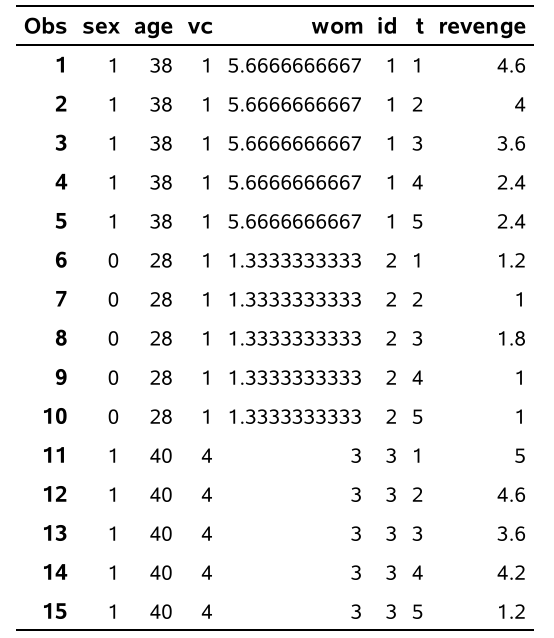
\includegraphics[width = 0.43\linewidth]{img/c5/slides6-e01}
\end{center}
\end{frame}

\begin{frame}
\frametitle{Evolution of desire for revenge  over time}
\bi
\item It's important to understand the \alert{structure} of the data, here ``one measurement per line''. 
\item Five lines in the file correspond to each individual.
\bi \item there are no missing values.
\item Each of the five line corresponds to a measurement time \code{t}.
\ei 
\item The only variable that changes over time is \code{revenge}. 
\bi \item The variables \code{sex}, \code{age}, \code{vc} and \code{wom} were only measured at time one, but they are repeated over each time point. 
\ei
\item For longitudinal models, it is often necessary to format the data so that each line corresponds to a measurement (long format).
\ei
\end{frame}

\begin{frame}[fragile]
\frametitle{Descriptive statistics with repeated measurements}
 We need to be careful if we want to get descriptive statistics for variables that do not vary with time, such as \code{sex}, \code{age}, \code{vc} et \code{wom}. 
\bi 
\item The sample average is correct only because we have the same number of observations $T=5$ for each individual.
\item On the other hand, its estimated standard error will be too small because the effective sample size $N=80$ is smaller than the number of measurements $NT=400$.
\ei
\end{frame}
\begin{frame}
\frametitle{Example calculation}
The average age of the $N=80$ participants is $\overline{\code{age}}= 42.075$ years
\bi
\item the standard deviation is $S=7.49$ and $\mathsf{se}(\overline{\code{age}})= 0.837$, where
\[S^2=\frac{\sum_{i=1}^N (\code{age}_i-\overline{\code{age}})^2}{N-1}, \qquad \mathsf{se}(\overline{\code{age}})=\frac{S}{\sqrt{80}}.\]
\ei
Contrast this with the following \textbf{incorrect calculation}
\[S^2_{*} = \frac{\sum_{i=1}^{NT} (\code{age}_i-\overline{\code{age}})^2}{(NT-1)} \approx S^2, \qquad \mathsf{se}(\overline{\code{age}}) \neq\frac{S_*}{\sqrt{400}} = 0.37 \]
\end{frame}
\begin{frame}[fragile]
\frametitle{Computing descriptive statistics}
If a variable is repeated over time, we can focus on a single time measurement.

\begin{tcolorbox}[colback=white, colframe=hecblue, title=\SASlang{} code to compute summary statistics]
\begin{small}
\begin{verbatim}
proc means data=statmod.revenge(where=(t=1)); 
var sex age vc wom; 
run; 
proc corr data=statmod.revenge(where=(t=1)); 
var sex age vc wom; 
run;
\end{verbatim}
\end{small}
\end{tcolorbox}

\end{frame}
% 
% \begin{frame}[fragile]
% \frametitle{Descriptive statistics for customer revenge}
% \bi
% \item We've seen the descriptive statistics for the four explanatory variables, but there's still a fifth one.
% \bi 
% \item the time variable,  $\code{t} \in\{1, 2, 3, 4, 5\}$.
% \ei
% \item  It could be that the desire for revenge increases (or decreases) at a certain rate through time. 
% \ei 
% \end{frame}
\begin{frame}[fragile]
\frametitle{Visualisation of time evolution}
\bi
\item It's possible that the desire for revenge changes over time. A simple way of visualizing the time evolution of desire for revenge is to plot \code{revenge} as a function of \code{t} \alert{for each individual}.
 \ei 
\begin{tcolorbox}[colback=white, colframe=hecblue, title=\SASlang{} code to draw a spaghetti plot]
{\small
\begin{verbatim}
proc sgplot data=statmod.revenge;
series x=t y=revenge / group=id;
run;
\end{verbatim}
}
\end{tcolorbox}

\end{frame}




\begin{frame}[fragile]
\frametitle{Spaghetti plot}
\begin{center}
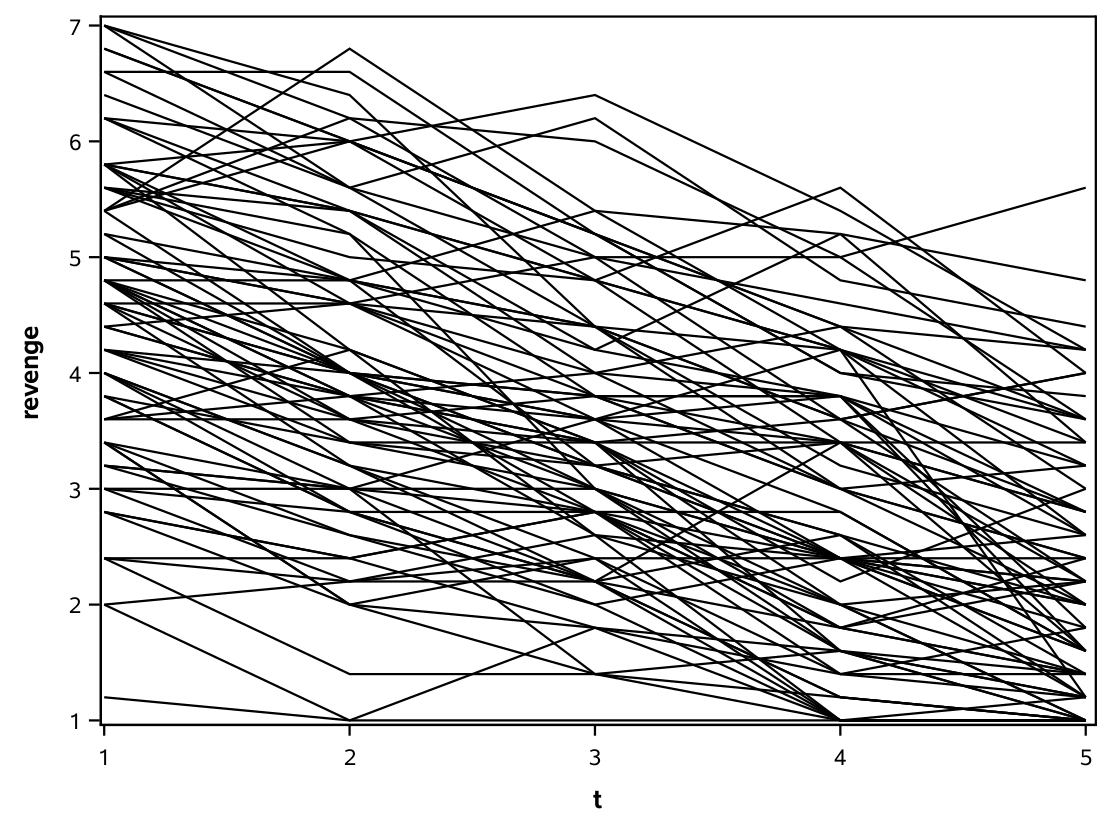
\includegraphics[width = 0.7\linewidth]{img/c5/slides6-e02}
\end{center}
This so-called spaghetti plot shows $80$ curves (one for each person). The desire for revenge value seems to decrease with time, on average.
% \end{frame}
% 
% \begin{frame}[fragile]
% \frametitle{Plot of revenge over time}
% 
% \begin{tcolorbox}[colback=white, colframe=hecblue, title=Plot of revenge over time for first $10$ individuals]
% {\small
% \begin{verbatim}
% proc sgplot data=statmod.revenge(where=(id<11));
% series x=t y=revenge / group=id LineAttrs= (pattern=1);
% run;
% \end{verbatim}
% }
% \end{tcolorbox}
% \begin{center}
% 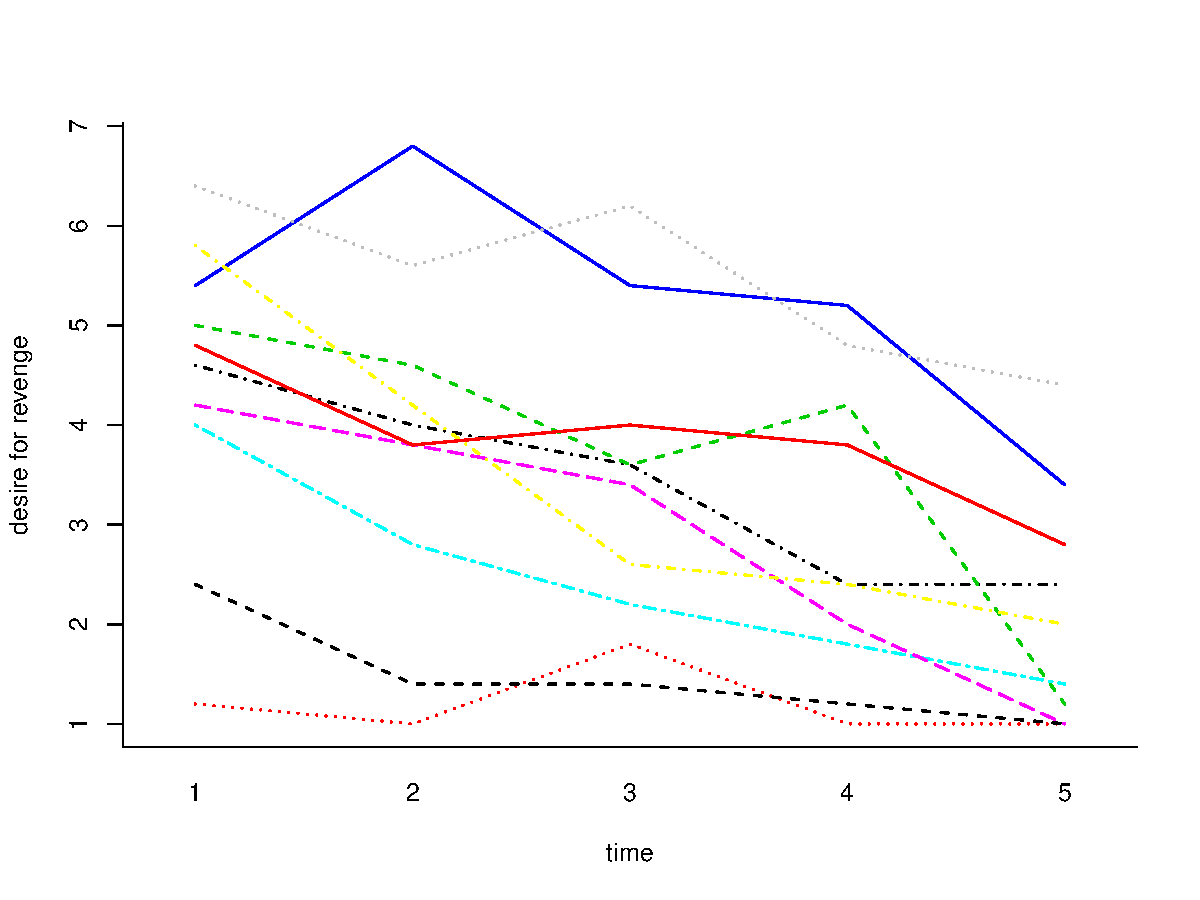
\includegraphics[width = 0.7\linewidth]{img/c5/06-correlated-spaghetti.pdf}
% \end{center}
The decrease in \code{revenge} through time could very well be linear. 

\end{frame}



\end{document}
